\section{Significance, Background, and Technical Approach}

RNET Technologies Inc. (RNET) in Dayton, OH and Oak Ridge National Laboratory 
(ORNL) are responding to 2019 DOE SBIR/STTR Phase II Release 2 
(DE-FOA-0001976). This proposal is for a Phase II contract in succession to an 
initial Phase I contract (Contract \#: DE-SC0018728) awarded for DOE 
SBIR/STTR Topic 30d (Modeling and Simulation). Based on a prototype developed in Phase I, RNET and ORNL are proposing the development of VnV: a self-documenting 
testing framework for in-situ solution verification and validation in high performance computing applications. In this proposal we will highlight the need for, and the tremendous value of, the proposed tool in high performance numerical simulations like those in the NEAMS toolkit. The goal of the proposed Phase II project will be to develop and demonstrate a production quality implementation of the VnV framework that can deliver this value to a broad spectrum of numerical simulation applications. 

\subsection{Identification and Significance of the Innovation}
\label{sec:identification}
%% {\em Define the specific technical problem or opportunity addressed by
%%  your application.  Provide enough background information so that the
%%  importance of the problem/opportunity is clear.  Indicate the overall
%%  technical approach to the problem/opportunity and the part that the
%%  proposed research plays in providing needed results.}

The fundamental concept of the VnV framework will be to facilitate the development of \emph{explainable} numerical simulations. That is, the VnV framework will equip developers with all the tools required to create simulations that not only provide a solution, but also a detailed description of how the solution was obtained and why it should be trusted. RNET has extensive SBIR experience in various aspects of High Performance Computing, including performance optimization of numerical softwares and libraries, development of fine-grained power monitoring tools for HPC infrastructure, and the development of software usability tools that enhance the user experience when working with HPC simulations. Dr. Watson, our collaborator at ORNL, is an experienced software professional with extensive knowledge of software design, architecture, and engineering practices. He has significant experience developing parallel debugging software for HPC environments, and  is the project leader of the open-source Eclipse Parallel Tools Platform project. We believe that our experience developing advanced numerical software for the HPC community combined with Dr. Watson's experience with scientific software engineering uniquely qualifies our team to fully develop and commercialize the VnV framework.

\subsubsection{Identification and Significance}
\label{intro}
Numerical modeling and simulation M\&S is almost always more economical than live testing and prototyping; a fact that has seen wide-scale uptake of M\&S in the R\&D lifecycles of products ranging from \$10 polycarbonate toys, up to solar panels, airplane wings and nuclear reactors. With access to large-scale computational resources at an all time high, and with exascale computing resources on the horizon; the role of \MS in the design of next generation technologies is only expected to increase. However, numerical simulations are, by definition, an \emph{approximation} to a real world physical system. As such, it is important that this increased reliance on simulated tests is accompanied by a concerted effort to ensure simulations are fit for the intended purpose.  As stated in the DoD best practices guide \cite{dodvv}, verification and validation (V\&V) of a code should be performed when  \emph{``...the risk of making an incorrect decision based on a simulation outweighs the time and cost of performing \VV to ensure that a simulation produces results that are sufficiently accurate and reliable.''} One only needs to look to the Sleipner platform accident, where an offshore oil platform collapsed due to failures in the finite element simulation, to get an idea of the devastating consequences poorly verified numerical simulations can have on business, the environment and society.

%The first \VV guideline was issued by the American Nuclear Society in 1987. Further development of \VV guidelines was conducted by other professional organizations to provide industry-specific standards. In 1998, the American Institute of Aeronautics and Astronautics (AIAA) released its first modern standards document. Thereafter, the American Society of Mechanics Engineers (ASME) \VV Standards Committee issued documents related to fluid dynamics and solid mechanics, including
%\begin{itemize}
% \item A Standard for Verification and Validation in Computational Fluid Dynamics and Heat Transfer, ASME \VV-20 (2009).
% \item An Illustration of the Concepts of Verification and Validation in Computational Solid Mechanics, ASME \VV-10.1 (2012). 
%\end{itemize}

The general concensus of these industry specific \VV reports is that \VV should be an iterative, integrated component of the software development lifecycle. The staples of a rigorous \VV regimen are:

\begin{itemize}
 \item The development of a detailed \VV plan
 \item The implementation of software development best practices (e.g. version control, unit and regression testing, code reviews, etc.)
 \item Mathematical and algorithmic testing (convergence analysis, mesh refinement studies, method of manufactured solutions, etc.)
 \item Development of a broad benchmark testing suite
 \item Uncertainty quantification and sensitivity analysis
 \item Comparison of simulation results with experimental data and results from third party simulations. 
 \item Review of the implementation and results by experts in the field
 \item Documentation of the \VV effort
\end{itemize}

\VV is a discrete process that cannot realistically account for each and every possibility. This raises significant issues in the development of general purpose numerical simulation packages because, while it may be the responsibility of the program developers of such packages to ensure that their product is mathematically correct and is free of programming errors (so-called bugs), it is ultimately the responsibility of the end user to ensure the solution obtained is an suitable representation of their physical model. After all, the direct costs of a design failure, be it time, money or loss of life, fall squarely on the shoulders on the products creator, and any attempt to shift the blame to the developers of simulation library $X$ will certainly fall of deaf ears. 

End-user \VV is of particular importance in the DOE Nuclear Energy Advanced Modeling and Simulation (NEAMS) program. NEAMS is developing predictive models for the advanced nuclear reactor and fuel cycle systems using leading edge computational methods and high performance computing technologies \cite{NEAMS}. An important objective of the NEAMS program is to enable widespread use among the industry, academia, and regulatory communities\cite{NEAMS}. This objective led to the development of the NEAMS workbench, which has significantly increased the overall user experience of the NEAMS tools. The NEAMS group has also placed a significant emphasis on \VV in the NEAMS toolkit, as outlined in the NEAMS \VV plan (version 0) \cite{neams-vv}. The result of this is that the NEAMS tools have integrated functionality for input validation (through the workbench and MOOSE), for performing mesh refinement and method of manufactured solution analysis (through MOOSE) and for completing uncertainty quantification and sensitivity analysis with DAKOTA (through the workbench). Despite this, the complex nature of the codes, combined with the expert knowledge required to set up \VV testing and the seemingly infinite array of input parameters (PETSc, the linear solver package used in MOOSE has hundreds of configuration options alone) makes setting up robust end-user \VV an complicated task for all but the most expert users.   

To address the difficulties with end user solution verification in the NEAMS toolkit, and the numerical simulation community as a whole, RNET Technologies Inc. (RNET) and Oak Ridge National Laboratory (ORNL) are proposing the development of the VnV toolkit; a C/C++ software package that facilitates end user \VV in general purpose numerical simulation packages (e.g., MOOSE, PETSc, libMesh, Fenics, OpenFoam, etc). To do this, the framework will promote the development of \emph{explainable} numerical simulations that, in addition to producing a simulation result, produce a detailed report outlining how the solution was obtained and why it should be trusted. 

%From the perspective of the DOE, the explainable numerical simulations promoted by the proposed framework will increase the appeal its government funded simulation technologies, drive technology transfer and help ensure the nation benefits from its significant investment in advanced numerical simulation technologies. Likewise, from a commercial perspective, the VnV framework is a mechanism for building trust in the results obtained from the product, while also making the simulation stand out in a very competitive market. 


\subsubsection{Product Overview and Technical Approach}

In this proposal, we make the distinction between \VV \emph{of} a simulation package and the end-user \VV of a solution obtained \emph{using} a simulation package. These two processes are not independent; indeed, \VV of a numerical simulation 
package almost always includes a set of verified and validated benchmark tests; likewise, the assertion that a package is verified and validated forms the foundation of trust in in solutions obtained by end-users. The focus of this proposal and the phase II project will be end-user validation; however, there is no reason that the functionality imparted by the proposed framework could not be used in the \VV process of the overall simulation package as well. 

They key issues associated with end-user verification and validation, and the approaches that the VnV framework will take to address them are:

\begin{itemize}
 
 \item{ \bf In-situ Testing And Analysis:} Unit tests are an extremely effective mechanism for ensuring a algorithm behaves as is expected. However, such testing is an unavoidably discrete process that, by definition, cannot cover every possible outcome. This fact is particularly true for numerical algorithms, where even small changes (e.g., input parameters, mesh geometry. etc.) can cause algorithms to behave unexpectedly (i.e., diverge, converge to the wrong solution, etc.). As such, a robust \VV report should not only include a description of unit tests completed, but also a detailed set of in-situ tests and assertions that run as the simulation proceeds. The VnV framework will include a sophisticated test injection system. At run time, the system will automatically detect, configure and assimilate data obtained from injection points in any VnV equipt library that is linked to the executable. For example, once fully integrated at all levels of the simulation heirarchy, the user of a MOOSE tool would be able to detect, configure, modify and run tests at injection points defined in the source codes of hypre, PETSc, libMesh, MOOSE, etc. This cross library support will allow for in-depth, expert directed, end-user \VV in executables that utilize a range of numerical simulation libraries. A key feature of the framework is that, while the injection points will hard coded into the source code of the individual libraries, the tests themselves are compiled in external shared libraries loaded at runtime based on a user specified configuration file. 
 
 \item {\bf Reusable Software Components:} While the specific details of \VV vary from application to application, the macro scale algorithms used are relatively consistent, including; mesh refinement studies, using the method of manufactured solutions, sensitivity analysis, uncertainty quantification and error propagation. Many of these algorithms can be, and in some cases already have been (e.g., DAKOTA, MASA),  implemented as black-box or near black box solutions. The VnV framework will look to capitalize on this fact by providing a set of robust, near black-box, \VV tools that can be integrated into codes using the VnV runtime test injection system. 
  
 \item{\bf \VV Testing Efficiency:}  Performing a large number of \VV tests in a distributed environment will be expensive, both computationally and due to the data movement required to deal with the domain decomposition employed by the application. Where possible, the VnV framework will offer functionality for offloading the execution of in-situ tests to external processes. Offloading of the tests to an external server will significantly reduce the run time costs of in-situ \VV with the VnV framework; further increasing its utility in HPC applications. 
 
 \item{\bf Documentation Generation:} With software packages under almost constant development, and new and improved packages being released on a regular basis, keeping an up-to-date \VV report is in an almost impossible task. The VnV toolkit will include automatic VnV report generation in the form of a server-less html web page that can be viewed in any modern web browser. The entire web page will be built using an extended markdown format with support for standard markdown formating, latex formating, images, videos, self-sorting tables, two dimensional charts, and three dimensional visualization. %The format of the overall web report will follow the templates outlined in the DMSCO Verification, Validation, \& Accreditation (VV\&A) reference sites template files for VV\&A reports. These templates have been used over many years in the \VVA of DoD simulations to great effect. Of course, additional custom templates will also be supported. 
 \end{itemize}

\begin{figure}
\centering
 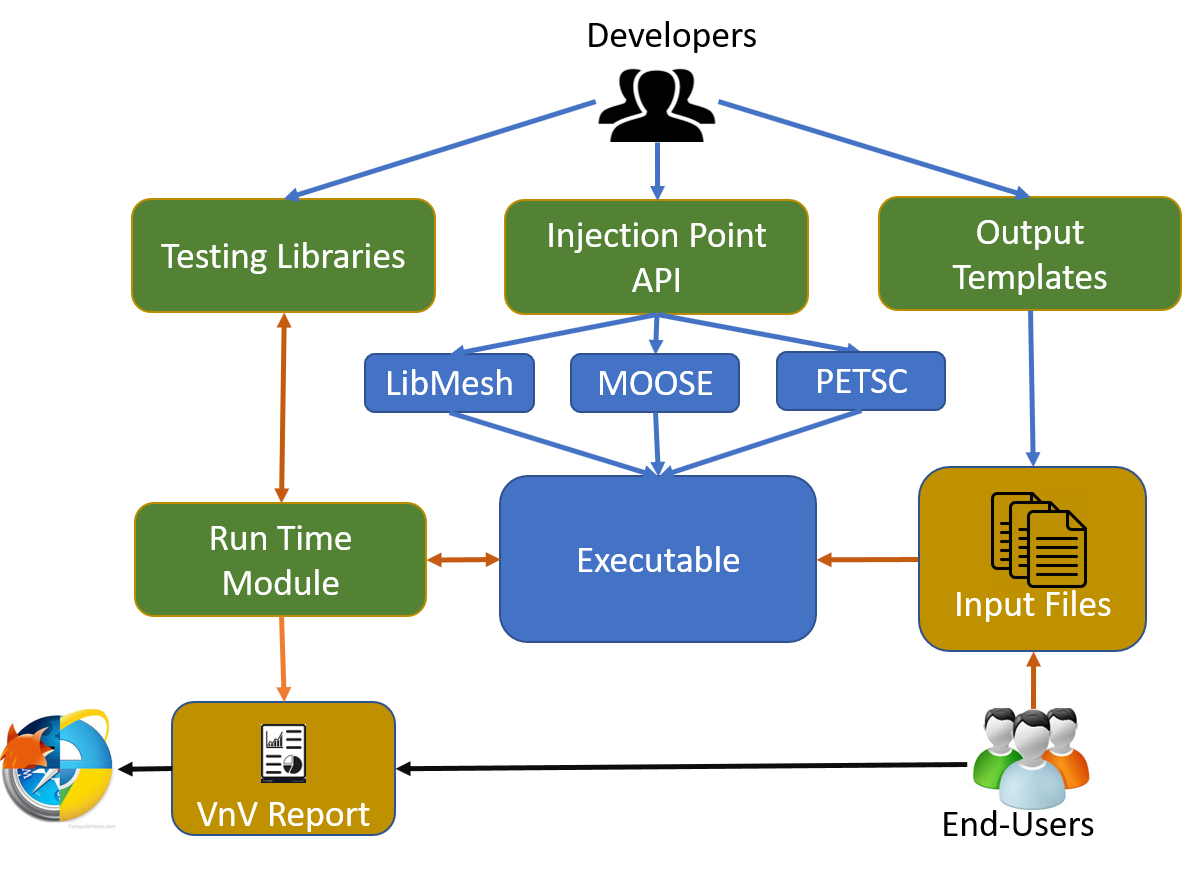
\includegraphics[width=0.7\textwidth]{./narrative/figures/VnVOut.png}
 \caption{ The VnV toolkit development lifecycle. Here, green boxes represent core VnV functionalities. Developer interactions are shown in blue, runtime interactions are shown in orange and post-processing interactions are shown in black. \label{fig:toolchain} } 
\end{figure}
 
Figure~\ref{fig:toolchain} provides an example of how developers and end-users will interact with the VnV toolkit. In this case, we show an example of how the toolkit functionality might be implemented in the MOOSE toolchain. The first step in the VnV development lifecycle is to specify and describe the injection points. These injection points will be placed at key locations of the code where testing can and should take place. In the Phase II product, inserting an injection point into a code will be as simple as annotating some variables for inspection and calling an injection point function. In addition to adding the code, developers will also complete an output template that will be used in the final \VV reports to describe the state of the simulation each time that injection point is met. The VnV tests are developed in external libraries and hence, can be developed either by the developer of the simulation or by the end-user of the code. The core framework will also include a robust set of general purpose \VV tests. We envision that the developers of a numerical simulation package will ship the library with hard-coded injection points, a set of custom \VV tests and a number of VnV configuration files. 

The end-users of the simulations will interact with VnV framework through the configuration files. Through a simple function call, users will be able to pre-generate a VnV configuration file that contains information about every injection point that is contained in any VnV enabled library in the simulation tool-chain. After customizing that file, generating a VnV report is as simple as running the simulation and opening the report in any web browser.
 
In summary, once integrated into an application, the VnV framework will provide a simple mechanism for creating self verifying, self describing, explainable numerical simulations. This will significantly reduce the burden associated with \VV for end user simulations, thereby increasing the usability of the tools for non-expert end-users. The framework will support a full range of in-situ \VV tests with functionality for offloading in-situ tests to external processors. Finally, the package will include support for generating a highly customizable, web-based \VV report. A commercial license will be required to incorporate the VnV toolkit into for profit applications; however, the core functionality of the VnV toolkit will be released as open source for use in academic and enterprise applications, with RNET providing commercial support, training and integration contracts to interested parties. 


\subsection{Anticipated Public Benefits}

The initial customers of the VnV framework will include the businesses and other institutions (e.g.,ANSYS, Cd-adapco, government labs, universities) that develop large-scale numerical models and simulations. To these customers, RNET will provide the training, support and integration services required to quickly and efficiently integrate the VnV framework into new and existing code bases, as well as contract based services for extending the toolkit to fit certain needs. For these customers, the benefits could include streamlining of the companies internal \VV practices, and an increase in the usability, reliability and confidence in their final product.

The true beneficiaries of the VnV framework are the users of the advanced numerical simulation products. By removing the burden associated with \VV, the VnV framework will ensure erroneous errors do not propagate into final designs. All in all, the VnV framework will afford researchers and engineers with the knowledge required to drive the next generation of technological advancements. 

\subsection{Phase I and Feasibility Demonstration}

The primary goal of the Phase I effort was to demonstrate the feasibility of in-situ end-user 
verification and validation of numerical simulations. To that end, the project team spent the majority of the Phase I
project developing an initial prototype that demonstrates the core functionality of the VnV toolkit.

\subsubsection{The VnV Injection Point System}

The core functionality of the injection point system was written in C++ with a focus on minimizing the amount of 
code required to integrate the injection points into existing code bases. Figure~\ref{fig:example} shows the three stages of specfiying an injection point; the declaration; the specification; and the final HTML rendering. In this case, the injection point is applied inside a class member function that evaluates a linear function at a particular value of $x$.

\begin{figure}
 \centering
 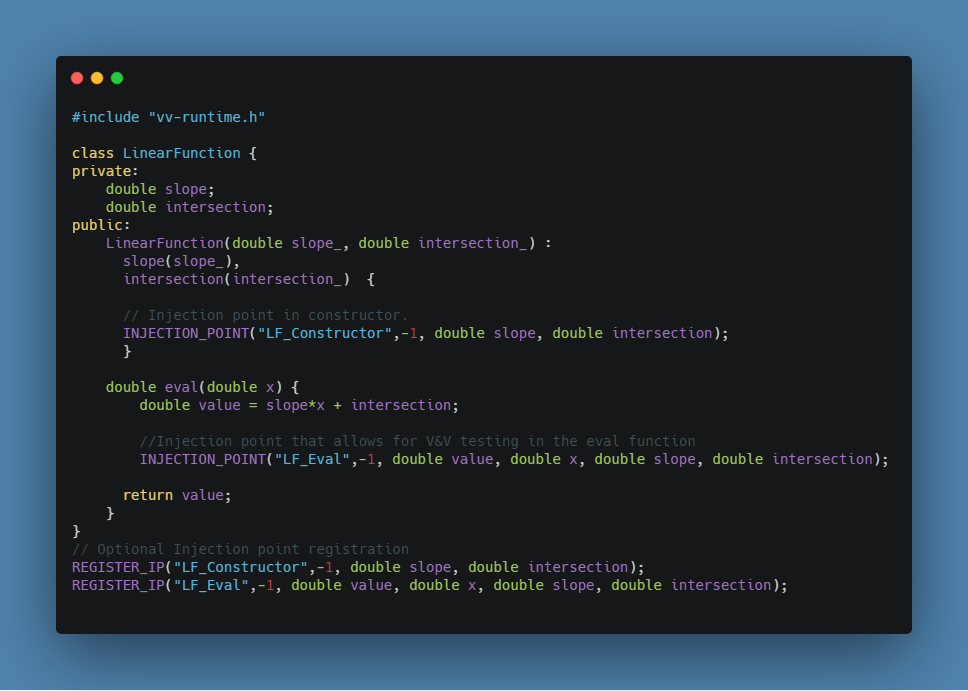
\includegraphics[width=0.65\textwidth]{./narrative/figures/code-example.png}
 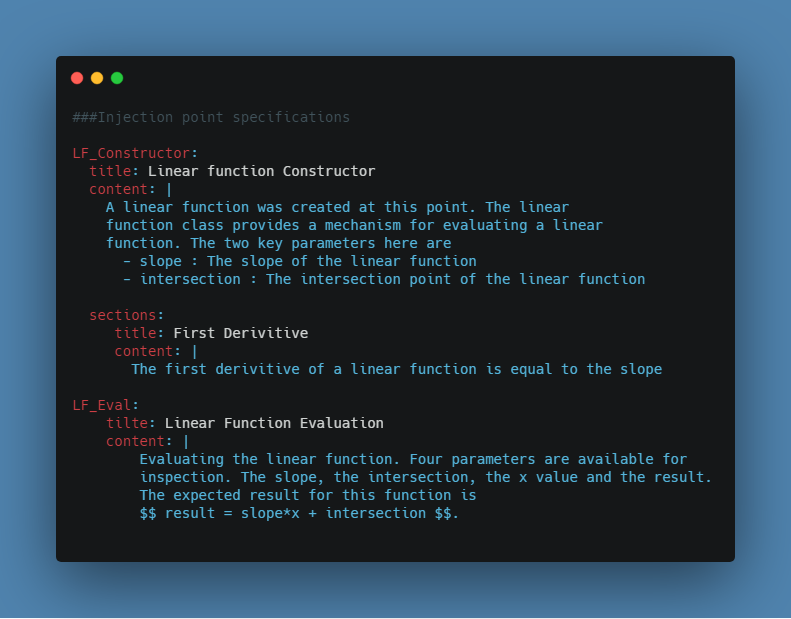
\includegraphics[width=0.65\textwidth]{./narrative/figures/template-example.png} 
 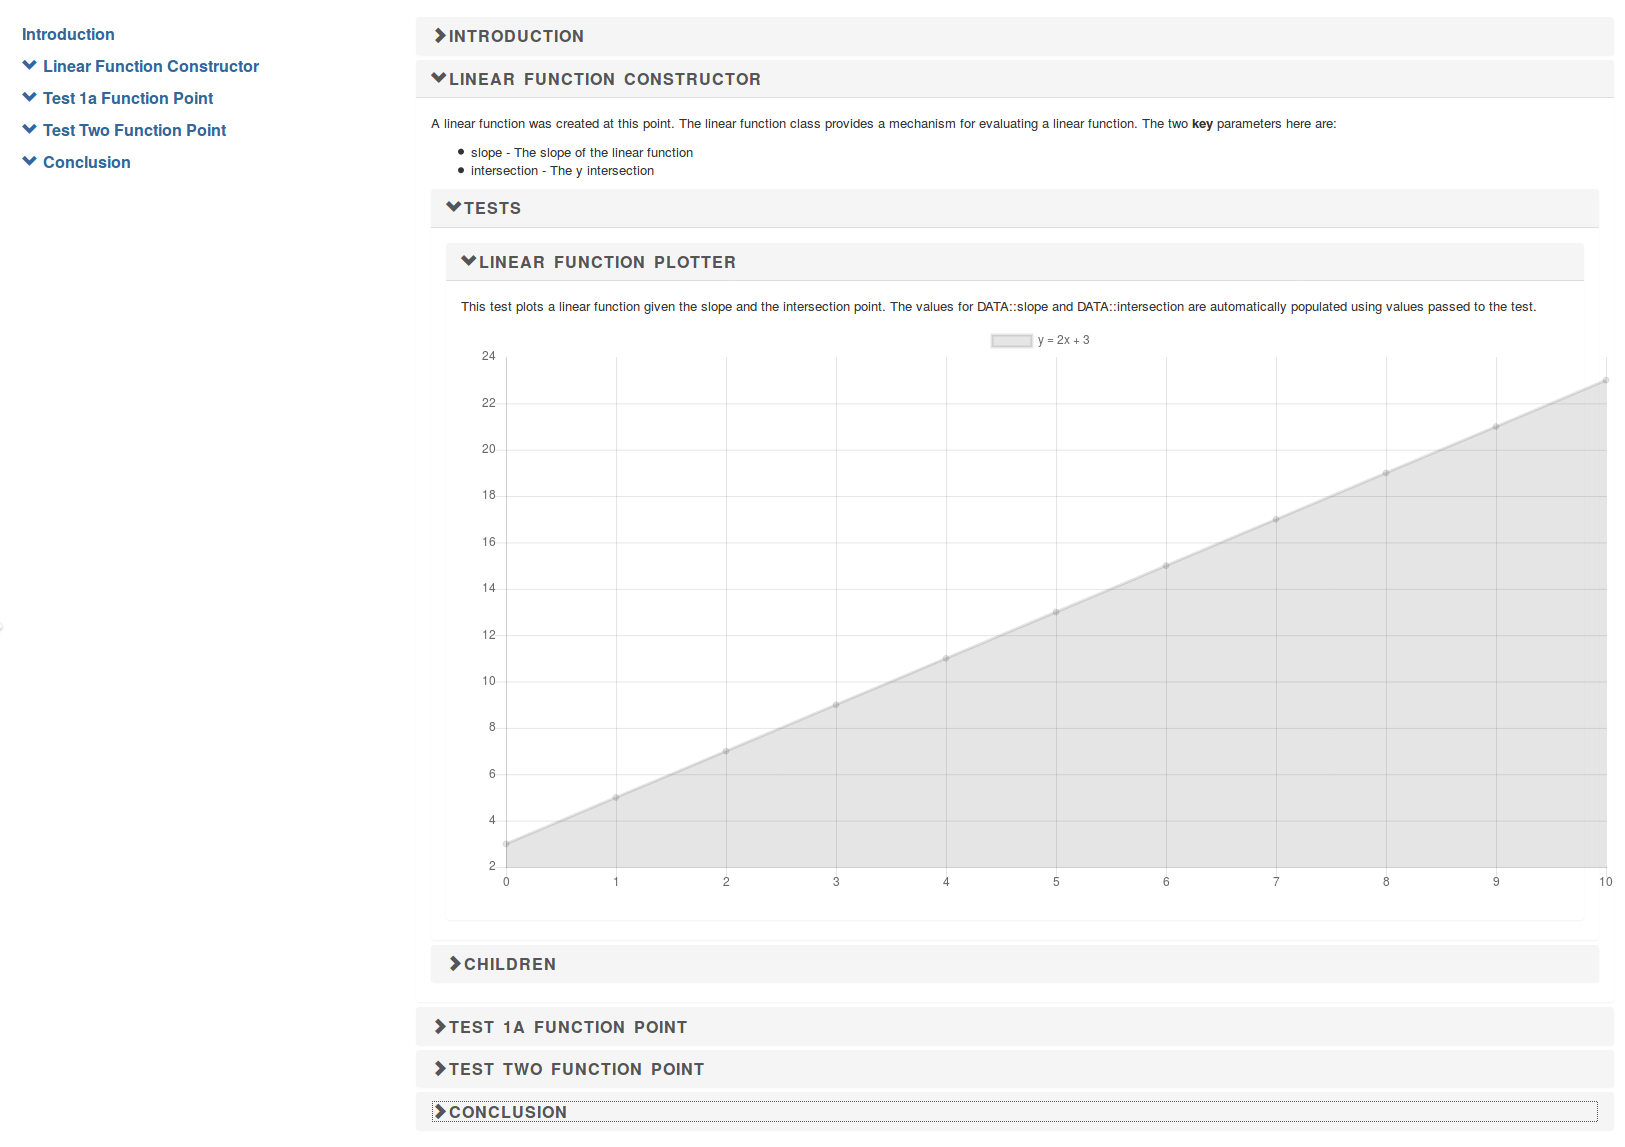
\includegraphics[width=0.65\textwidth]{./narrative/figures/render-example.PNG}
 \caption{Sample code showing two injection points inserted into a C++ class that represents a linear functions. Top: The source code modifications required to specify an injection point. Middle: The injection point specification written using the custom markdown extension; Bottom: The final rendering of the injection point in the VnV report. \label{fig:example}}
\end{figure}


Integration of an injection point into an existing code is a simple, three step process; (1) include the ``vv-runtime.h'' header file, (2) place injection points in the code and (3) write the injection point specification. 

At the core of the system is the INJECTION\_POINT macro. The format for this macro is:

\begin{verbatim} 
INJECTION_POINT( <name>, <stage>, <type> <variable>, ...)
\end{verbatim}

Here, ``name'' is the id that will be used to define the injection point in the configuration files and the final reports. This name must 
be unique across all injection points in an executable. The stage parameter is an integer value that defines the step that this injection point belongs to. Using this parameter, the developer can set up multi-staged injection point testing. Tests defined on staged injection points stay in scope across 
all stages allowing for data collection across multiple code locations. The variable parameters allows the develop to specify which variables can be inspected and tested at each injection point. The phase I prototype uses a combination of string based type checking, static casts to (void*) and C style variadic function calls to achieve this task. To enter a variable, the developer must pass the type and the variable to the macro. When the function is called at runtime, the VnV injection point factory compares the types accepted by the specified tests against the type specified at the injection point. There are several risks associated with this approach, the most important of which is memory corruption from a bad cast. A key goal of the Phase II project will be to develop a set of custom preprocessor directives that use compile time checks to minimize these risks. (see Section~\ref{sec:workplan}).

The final step in the creation of an injection point is to write the injection point specification. The specification is a YAML file containing the content used to populate the final VnV report (see Figure~\ref{fig:example1}). The only required parameter in the specification is the name; however, the more information that is entered here, the more informative the final report will be. The content entry represents the text that will be shown in the final report each time the code reaches the associated injection point. This content is specified  using a custom markdown format that supports all standard markdown commands, along with a range of data visualization extensions (described below). 

The second facet of the injection point system are the specific \VV tests. The development of the 
test interface was based on the idea that tests should be loaded at runtime and defined independently of the source code. To achieve this, the test interface was built using a C++ plugin pattern. 

The first step in the development of a new VnV test is to create a testing library. The framework includes a library generation script that will automatically build the directory structure and makefiles required to 
build this library. All that is required of the user for this step is to call this script with a unique name. 

Once the library has been initialized, the user can begin to develop individual tests. Writing a test is as simple as implementing the IVVTest Interface. To assist in the development of tests, and to avoid issues with incorrect type-casting, a python based test generation script is created as part of the library initialization step. This script can be used to automatically generate the boiler plate code required to implement the testing interface while also taking care of the required typecasting. 


\begin{figure}
 \centering
 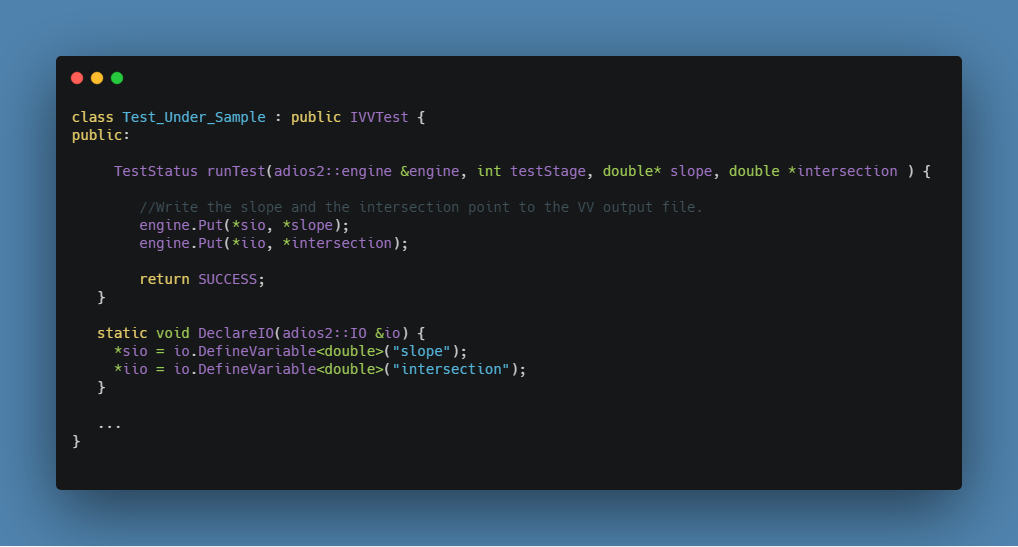
\includegraphics[width=0.45\textwidth]{./narrative/figures/testcode-example.png}
 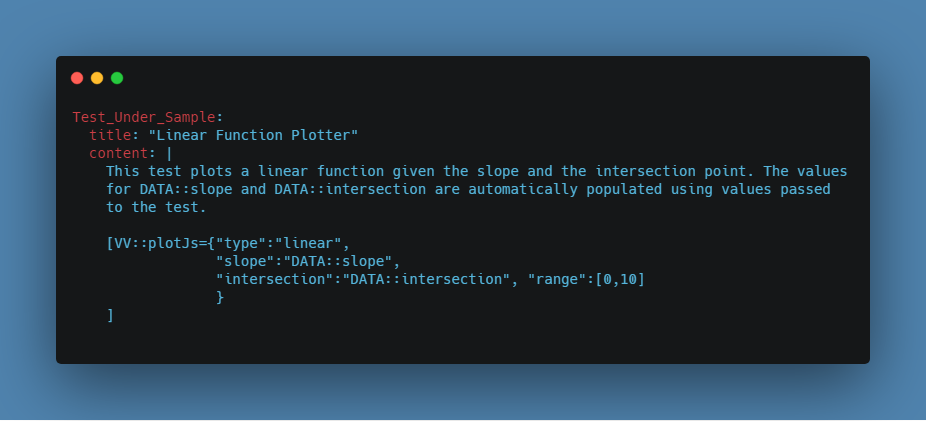
\includegraphics[width=0.45\textwidth]{./narrative/figures/test-example.png} 
 \caption{Sample code a custom VnV test for tracking the slope and intersection point of a linear function. \label{fig:test-example}}
\end{figure}


Implementing the IVVTest interface is a three step process. First, the developer must define the names and types of the parameters the test will support. This is completed in the constructor by adding the name and type of certain parameters to the parameters list. The only requirement on parameters is that the names should be unique within the test. To ensure efficiency in HPC settings, the VnV framework uses ADIOS for all data output. Writing data inside a test using ADIOS is a two step process that requires the user to (1) declare the output variables that will be written and (2) write the data. Tests should declare the output variables in the DeclareIO function. Note that it is not a requirement that the output variables be defined in advance, however it is good practice and allows for more efficient handling of the meta-data in ADIOS. The actual testing and writing of the data should occur in the runTest function. The variables passed to the test are direct pointers to the variables in the code. Hence, tests should not modify the pointers in any way; however, the phase I prototype does not strictly enforce this requirement. Beyond that requirement, there is not limit on the procedures that can be run inside a test. 

As with the injection points, the final step in the test creation process is to define the test specification. This specification acts as the link between the data collected during testing and the final report. Figure~\ref{fig:test-example} shows an example specification for a test designed to verify and validate the slope and intersection point of a linear function. The test specification uses the custom extended markdown format to automatically populate and render an interactive line chart representing the linear function. This specification was used to render the ``Linear Function Plotter'' section shown in Figure~\ref{fig:example1}

Our vision for the VnV toolkit is that each numerical library will ship with hard-coded injection points and a custom VnV Testing library. The core VnV framework will act as a single interface to these individual libraries, allowing the end-users to build explainable numerical simulations with integrated, in-situ testing at every level of simulation hierarchy. 

Once the injection points have been declared and the tests created, the next step is to develop the XML test configuration file. Using this XML file, users can configure which testing libraries to load and which tests to run. Please see the final report for a full description of the XML format supported by the phase I prototype. 

With the configuration file in hand, performing VnV in a simulation is as simple as including a header file, linking the VnV library and calling the VnV Initialization function. 

\subsubsection{Automated Report Generation}

At the core of the report generation system is a custom markdown extension. This extension supports a range of custom data visualization features that interact directly with the output data in the ADIOS2 output file. For example, the chart shown in  Figure~\ref{fig:example} utilizes the support for generating two dimensional plots using the format. Other functionality supported includes 3D visualization with VTK.js and interactive tables with tabular.js. The extension also includes support for custom post-processing scripts. This allows for infinite possibilities with regard to processing the test outputs. For example, it is possible to  run a paraview script that generates VTI files based on the test data. 

\rnetcomment{TODO}
Figures~\ref{TODO} show screen-shots of a sample VnV report generated using a set of toy testing libraries. The main layout consists of three components; the carousel, the index and the content. The carousel is an optional component that can be used to highlight important results of the simulation. It accepts up to ten pictures, each with its own custom caption. The index and content are generated automatically based on the VnV output file. Each node in the index represents an injection point encountered during the simulation. As such, this index represents a coarse grained view of the simulations call stack. At the top of each injection point section is the injection point content as specified in the injection point specification. Following this is the output of each test completed at the injection point. Last is the list of children. These children represent injection points that were initialized between the first and last step of a staged injection point. %A live version of this sample VnV report will be available at http://www.rnet-tech.net/VV/sample.html until the date of award notification. 

\subsubsection{ Demonstration in a Moose Application } 
To demonstrate the utility of the method, the project team placed several injection points 
in the main function of a MOOSE example ``ex01'', one injection point in the PETSc Initialize function and 
one injection point in the PETSc Finalize functions. This is an extremely simple example that 
did not test the full limits of the new API; however, it did act to verify that the phase I prototype 
can be used to can be used to perform in-situ verification and validation in a across multiple libraries 
through a single interface. 

In summary, during Phase I, the project team created a functioning prototype of the VnV framework that provides:
\begin{itemize}
 \item A clean mechanism for inserting injection points in existing codes
 \item A simple interface for defining custom tests 
 \item A python based report generation code that automatically creates an interactive server-less web report based on the VnV output.
\end{itemize}

As will be described in the workplan, the goal of the Phase II project will be to take this initial prototype and extend, harden and 
optimize it such that it can be efficiently used in high performance computing applications. 





























